\documentclass{article}

\usepackage[final]{neurips_2020}

\usepackage[utf8]{inputenc}
\usepackage[T1]{fontenc}
\usepackage{hyperref}
\usepackage{url}
\usepackage{booktabs}
\usepackage{amsfonts}
\usepackage{nicefrac}
\usepackage{microtype}
\usepackage{graphicx}
\usepackage{xcolor}
\usepackage{lipsum}
\usepackage{float}

\newcommand{\note}[1]{\textcolor{blue}{{#1}}}

\title{
  Ko-Binoculars: Zero-Shot Detection of AI-Generated Korean Text via NLL Dispersion Calibration \\
  \vspace{1em}
  \small{\normalfont Korea University COSE461 Final Project}  % Select one and delete the other
}

\author{
  GyeongMin Bae \\
   Department of Artificial intelligent \\
   Team 14 \\
   2025320605
  \And
  SeongHyeon Mun \\
  Department of Computer Science \\
  Team 14 \\
  2020320012
}

\begin{document}

\maketitle

\begin{abstract}
Detecting AI-generated text has become increasingly important as large language models (LLMs) produce text nearly indistinguishable from human writing. Although zero-shot detection methods such as Binoculars have shown strong performance in English, their effectiveness on non-English languages remains limited. In this work, we present Ko-Binoculars, a zero-shot framework for detecting AI-generated Korean text. We first demonstrate that replacing English-centric models with Korean-optimized observer-performer pairs improves ROC-AUC from 67.54 to 95.40 on the KatFish benchmark. We then propose NLL Dispersion Calibration, a training-free method that leverages the observation that AI-generated text exhibits significantly lower token-level NLL variance than human text. By multiplicatively calibrating the Binoculars score with a z-score derived from NLL dispersion, we achieve an additional +2.44 ROC-AUC improvement. We provide theoretical grounding for this observation by demonstrating a strong correlation between NLL dispersion and sampling temperature (r = 0.73), and estimate that human text corresponds to an effective temperature of 1.38 while AI text ranges from 1.05 to 1.11. Finally, we extend our framework to segment-level detection, estimating the proportion of AI-generated content within mixed documents with a 45.7\% lower error than random baseline. Our results demonstrate that effective zero-shot AI text detection for non-English languages is achievable through principled model selection and statistical calibration, without requiring any training data.
\end{abstract}


\section{Introduction}
The rapid advancement of LLMs has made it increasingly difficult to distinguish AI-generated text from human writing, motivating the need for reliable detection methods. As a result, reliable detection methods for AI-generated text have become a pressing research need.

Among existing detection approaches, Binoculars~\cite{hans2024binoculars} stands out as a promising zero-shot method that requires no additional training data. By computing the ratio of perplexity to cross-perplexity using two language models (an observer and a performer), Binoculars achieves over 0.90 AUC on English benchmarks. However, the original method relies on English-centric models (Falcon-7B~\cite{penedo2023falcon}), and its performance degrades substantially in low-resource languages. For Korean, the original Binoculars achieves only 67.54 ROC-AUC on the KatFish benchmark~\cite{park2025katfishnet}, far below practical applicability.

On the other hand, KatFishNet~\cite{park2025katfishnet} achieves strong performance on Korean AI-text detection (97.57 ROC-AUC), but relies on supervised training and large-scale labeled data, requiring retraining for newly released models.

In this work, we present Ko-Binoculars, a framework for zero-shot detection of AI-generated Korean text that addresses both limitations. Our contributions are threefold:

(1) Korean-optimized model replacement. We systematically evaluate five observer-performer model pairs on the KatFish benchmark, demonstrating that replacing English-centric models with Korean-optimized models improves ROC-AUC from 67.54 to 95.40 without any training.

(2) NLL Dispersion Calibration. We discover that AI-generated text exhibits significantly lower token-level NLL (negative log-likelihood) variance compared to human text, reflecting the uniform sampling behavior of LLMs. Based on this observation, we propose a multiplicative calibration method that adjusts the Binoculars score using the NLL standard deviation, achieving a modest but consistent improvement of +2.44 ROC-AUC on essay and poetry genres while maintaining zero-shot applicability. We note that this calibration does not improve performance on the abstract genre, where human and AI writing styles are statistically indistinguishable. We further validate this finding through the lens of sampling temperature, showing a strong correlation between temperature and NLL dispersion (r = 0.73, p < 0.0001).

(3) Segment-level detection. We extend document-level binary classification to segment-level detection, estimating the proportion of AI-generated content within a mixed document. Using a sliding window approach with soft scoring, our method achieves a 45.7\% lower estimation error compared to the random baseline, with robustness to insertion position.

Our framework is evaluated on the KatFish dataset~\cite{park2025katfishnet}, a Korean AI text detection benchmark spanning three genres (essay, abstract, poetry) and four generative models (GPT-4o~\cite{openai2024gpt4o}, Solar~\cite{kim2024solar}, Qwen2~\cite{yang2024qwen2}, Llama3.1~\cite{dubey2024llama}). The results show that Ko-Binoculars with NLL Dispersion Calibration achieves competitive performance with supervised methods while requiring no training data, demonstrating the viability of zero-shot detection for non-English languages.

\section{Related Work}

\textbf{Zero-shot AI text detection.} Zero-shot methods detect AI-generated text without requiring labeled training data, relying instead on statistical properties of language model outputs. Early approaches used simple metrics such as log-likelihood, rank, and entropy of token predictions to distinguish human from machine text~\cite{solaiman2019release, gehrmann2019gltr, ippolito2020automatic}. DetectGPT \cite{mitchell2023detectgpt} introduced perturbation-based detection, measuring the curvature of the log-probability function around the input text. Fast-DetectGPT \cite{bao2024fastdetectgpt} improved upon this by replacing random perturbations with conditional sampling, achieving significant speedups. Binoculars \cite{hans2024binoculars} proposed a novel metric based on the ratio of perplexity to cross-perplexity computed using two language models --- an observer and a performer. This approach achieved state-of-the-art English detection performance (AUC $>$ 0.90) with no training required. However, the original Binoculars relies on English-centric Falcon models~\cite{penedo2023falcon}, and the authors acknowledged that recall is low for low-resource languages such as Korean.

\textbf{Korean AI text detection.} KatFishNet \cite{park2025katfishnet} addressed the gap in Korean AI text detection by introducing KatFish, the first Korean-language benchmark dataset for AI-generated text detection, spanning three genres (essay, abstract, poetry) and multiple generative models. KatFishNet extracts Korean-specific linguistic features --- including spacing error rates, POS tag diversity, and punctuation patterns --- and trains a classifier on these features. Although it achieves strong performance (97.57 ROC-AUC), this supervised approach requires large-scale labeled data and retraining when new generative models emerge, limiting its practical deployment.

\textbf{Multi-feature fusion for detection.} MFD \cite{wu2023mfd} proposed a zero-shot detection method that combines multiple statistical signals (log-likelihood, log-rank, entropy, and LLM-Deviation) into a unified score, demonstrating that complementary metrics can improve detection accuracy. However, it has only been evaluated on English text. Our work shares the motivation of combining multiple statistical signals but differs in that we specifically address the challenges of Korean as an agglutinative language, and perform fusion through multiplicative calibration rather than simple score combination.

\section{Approach}

\subsection{Baseline: Ko-Binoculars}

Our work is based on Binoculars~\cite{hans2024binoculars}, a zero-shot AI text detection framework that compares perplexity and cross-perplexity between two language models: an observer model and a performer model.

Given an input text \(X\), Binoculars computes a detection score based on the ratio between perplexity and cross-perplexity:

\[
B(X)=\frac{\mathrm{PPL}(X)}{\mathrm{XPPL}(X)}
\]

where:

\begin{itemize}
    \item \(\mathrm{PPL}(X)\): perplexity computed by the performer model
    \item \(\mathrm{XPPL}(X)\): cross-perplexity computed using the observer-performer pair
\end{itemize}

Unlike the original English-centric Binoculars framework, we replace Falcon-based models with Korean-optimized observer-performer pairs. We systematically evaluate multiple Korean language models and select the best-performing pair on the KatFish benchmark.

This component was implemented by adapting the original Binoculars codebase and extending it for Korean language evaluation.

To guide model selection, we measure tokenizer fertility---the average number of tokens produced per character---for each observer model. English-centric models such as Falcon-7B~\cite{penedo2023falcon} exhibit high fertility (2.13 tokens per character) on Korean text, indicating inefficient tokenization. In contrast, Korean-optimized models achieve substantially lower fertility (0.53--0.68), reflecting better coverage of Korean vocabulary. Although the small number of evaluated models ($n=4$) precludes formal statistical significance testing, we observe a consistent negative trend between tokenizer fertility and detection performance. This suggests that tokenizer efficiency may serve as a practical heuristic for model selection when extending zero-shot detection to new languages.

\subsection{NLL Dispersion Analysis}

We additionally analyze token-level negative log-likelihood (NLL) variance.

For each text \(X\), we compute the standard deviation of token-level NLL values:

\[
D(X)=\mathrm{std}(\mathrm{NLL}_1,\mathrm{NLL}_2,\dots,\mathrm{NLL}_n)
\]

where \(\mathrm{NLL}_i\) is the token-level negative log-likelihood for token \(i\).

Our hypothesis is that AI-generated text tends to exhibit lower token-level dispersion than human-written text because LLM sampling produces more uniform token probability distributions.

To normalize the dispersion signal, we compute a Human-based z-score:

\[
z(D(X))=\frac{D(X)-\mu_H}{\sigma_H}
\]

where:

\begin{itemize}
    \item \(\mu_H\): mean NLL dispersion of Human text
    \item \(\sigma_H\): standard deviation of Human NLL dispersion
\end{itemize}

We provide theoretical grounding for the effectiveness of NLL dispersion as a detection signal by investigating its relationship with sampling temperature. During text generation, LLMs sample tokens from a probability distribution controlled by a temperature parameter $\tau$. Lower temperatures produce more deterministic outputs, while higher temperatures increase randomness. We hypothesize that $D(X)$ reflects the effective temperature at which a text was generated. To validate this, we generate texts at 15 temperature settings ($\tau \in [0.1, 1.5]$ with step 0.1) and measure the resulting NLL dispersion. We observe a strong positive correlation (Pearson $r = 0.73$, $p < 0.0001$), confirming that NLL dispersion generally increases with sampling temperature, consistent with the interpretation that it captures generation uncertainty. Using the fitted regression, we estimate that human text corresponds to an effective temperature of 1.38, while AI-generated text in the KatFish dataset corresponds to approximately 1.05--1.11.

\subsection{Multiplicative Calibration}

Based on the observation that NLL dispersion correlates with generation uncertainty, we propose a training-free multiplicative calibration method.

Our final calibrated score is defined as:

\[
S(X)=Norm(B(X))\cdot \exp(-\lambda z(D(X)))
\]

where:

\begin{itemize}
    \item \(Norm(B(X))\): Min-Max normalized Binoculars score
    \item \(z(D(X))\): Human-normalized NLL dispersion z-score
    \item \(\lambda\): calibration strength hyperparameter
\end{itemize}

This formulation preserves the zero-shot nature of Binoculars while adaptively calibrating confidence using uncertainty-related signals.

We also experiment with a linear variant:

\[
S(X)=Norm(B(X))\cdot (1-\lambda z(D(X)))
\]

but found the exponential form to be more stable in practice.

\subsection{Gated Fusion}

To further explore adaptive uncertainty-aware fusion, we experiment with a gated fusion mechanism.

The gated score is defined as:

\[
S(X)=w(X)\cdot Norm(B(X))
+(1-w(X))\cdot Norm(D(X))
\]

where:

\[
w(X)=1-\sigma(\gamma |z(D(X))|)
\]

and \(\sigma(\cdot)\) denotes the sigmoid function.

In this formulation:

\begin{itemize}
    \item low \(|z|\): rely more on Binoculars
    \item high \(|z|\): rely more on NLL dispersion
\end{itemize}

Unlike multiplicative calibration, gated fusion dynamically adjusts the contribution of complementary signals on a per-sample basis.

We emphasize that our approach remains fully zero-shot and does not require any supervised training.

\subsection{Segment-level Detection}

Existing detection methods operate at the document level, classifying an entire text as either human-written or AI-generated. However, in real-world scenarios such as academic integrity verification, documents often contain a mixture of human and AI-generated content.

We extend Ko-Binoculars to segment-level detection using a sliding window approach. Given an input text $X$, we compute Binoculars scores for overlapping windows of $W$ tokens with stride $S$. Each window score is normalized relative to human and AI reference distributions, and the estimated AI ratio is computed as:

$$\hat{r} = 1 - \frac{1}{N} \sum_{i=1}^{N} \max\left(0, \min\left(1, \frac{b_i - \mu_{AI}}{\mu_{Human} - \mu_{AI}}\right)\right)$$

where $b_i$ is the Binoculars score for window $i$ and $N$ is the total number of windows. We set $W = 100$ and $S = 50$ in our experiments.

\section{Experiments}

\subsection{Data}

We evaluate our framework on the KatFish benchmark~\cite{park2025katfishnet}, the first Korean-language dataset for AI-generated text detection. Dataset statistics are summarized in Table~\ref{tab:dataset}.

\subsection{Implementation Details}

All experiments are conducted on a single NVIDIA A100-SXM4-40GB GPU. We evaluate five observer-performer model pairs: Falcon-7B + Falcon-7B-Instruct~\cite{penedo2023falcon} (original Binoculars), Polyglot-Ko 1.3B + 3.8B~\cite{ko2023polyglot}, EXAONE 2.4B + 7.8B~\cite{lgai2024exaone}, Qwen2.5-7B base + instruct~\cite{yang2024qwen2}, and Qwen2.5-3B base + instruct~\cite{yang2024qwen2}. For NLL dispersion calibration, we compute human reference statistics ($\mu_H = 2.41$, $\sigma_H = 0.31$) from the human test set. Calibration strength is evaluated over $\lambda \in \{0.1, 0.2, 0.3, 0.5, 0.7, 1.0\}$, and gating strength over $\gamma \in \{0.3, 0.5, 1.0, 1.5, 2.0, 3.0, 5.0\}$. All Binoculars and NLL dispersion scores are normalized using Min-Max scaling. For segment-level detection, we use a sliding window of $W = 100$ tokens with stride $S = 50$. No supervised training is performed at any stage.

\subsection{Results}

\subsubsection{Ko-Binoculars Baseline}

Table~\ref{tab:model_pairs} shows the detection performance across five observer-performer pairs. Replacing the English-centric Falcon models with Korean-optimized models yields dramatic improvements: Polyglot-Ko achieves 96.62 ROC-AUC, a gain of +29.08 over the original Binoculars (67.54). All four Korean-optimized pairs surpass 93 ROC-AUC, demonstrating that model selection is the primary factor in cross-lingual adaptation. Notably, the training-free Ko-Binoculars variants approach the performance of the supervised KatFishNet (97.57) while requiring no labeled data.

\begin{table}[H]
\centering
\caption{\textbf{Ko-Binoculars performance across observer-performer pairs.} All Ko-Binoculars variants are training-free. KatFishNet requires supervised training. Evaluation follows the OOD protocol described in Section 4.1.}
\label{tab:model_pairs}
\begin{tabular}{llcccc}
\toprule
Method & Training & ROC-AUC & PR-AUC & R@FPR5\% & F1 \\
\midrule
Falcon-7B + Instruct & $\times$ & 67.54 & 41.00 & 66.48 & 55.27 \\
Polyglot-Ko 1.3B + 3.8B & $\times$ & 96.62 & 66.65 & 75.60 & 65.27 \\
EXAONE 2.4B + 7.8B & $\times$ & 94.41 & 70.46 & 79.74 & 82.95 \\
Qwen2.5-7B base + inst. & $\times$ & 93.79 & 51.75 & 84.60 & 83.19 \\
Qwen2.5-3B base + inst. & $\times$ & 95.40 & 52.69 & 86.56 & 85.65 \\
\midrule
KatFishNet (Punct.) & $\checkmark$ & 97.57 & 78.99 & 62.65 & 94.88 \\
\bottomrule
\end{tabular}
\end{table}

\subsubsection{NLL Dispersion Calibration}

Table~\ref{tab:calibration_llm} presents the effect of multiplicative calibration on per-LLM detection performance using the Qwen2.5-3B pair. Calibration improves average ROC-AUC by +2.55, with the largest gain on Qwen2 (+5.74). We also evaluate gated fusion, which achieves comparable overall performance (+2.66) while adaptively adjusting signal contributions per sample. Both methods are training-free, requiring only human reference statistics.

\begin{table}[h]
\centering
\caption{\textbf{Per-LLM ROC-AUC with calibration and gated fusion (Qwen2.5-3B).} Calibration uses $\lambda = 0.5$, Gated uses $\gamma = 1.0$. Both are training-free.}
\label{tab:calibration_llm}
\begin{tabular}{lcccc}
\toprule
Method & Solar & Qwen2 & Llama3.1 & Avg \\
\midrule
Bino only & 89.46 & 82.78 & 84.29 & 85.51 \\
+ Calibration & 88.87 & 88.52 & 86.77 & 88.06 \\
+ Gated Fusion & 88.75 & 88.94 & 86.82 & 88.17 \\
\bottomrule
\end{tabular}
\end{table}

Table~\ref{tab:lambda} shows the calibration strength ablation. The exponential form consistently outperforms the linear variant, and performance is stable across $\lambda \in [0.3, 0.7]$, indicating robustness to hyperparameter choice.

\begin{table}[h]
\centering
\caption{\textbf{Calibration strength ablation.} ROC-AUC for linear and exponential calibration across $\lambda$ values. Baseline (Bino only, full evaluation set): 85.70. This differs from the per-LLM average of 85.51 in Table~\ref{tab:calibration_llm} due to varying class ratios across target LLMs.}
\label{tab:lambda}
\begin{tabular}{ccc}
\toprule
$\lambda$ & Linear & Exp \\
\midrule
0.1 & 87.05 & 87.11 \\
0.2 & 87.60 & 87.71 \\
0.3 & 87.87 & 88.03 \\
0.5 & 87.99 & 88.14 \\
0.7 & 87.99 & 88.10 \\
1.0 & 87.88 & 88.01 \\
\bottomrule
\end{tabular}
\end{table}

\subsubsection{Genre-wise Analysis}

Table~\ref{tab:genre} reports genre-wise performance. Calibration and gated fusion yield substantial improvements on essay (+2.94 / +3.34) and poetry (+5.97 / +6.30). However, abstract detection remains challenging, with performance below the Binoculars baseline. We analyze this limitation in Section 5.

\begin{table}[h]
\centering
\caption{\textbf{Genre-wise ROC-AUC (Qwen2.5-3B).} Essay and poetry benefit from calibration. Abstract remains challenging due to stylistic uniformity between human and AI academic writing.}
\label{tab:genre}
\begin{tabular}{lccc}
\toprule
Genre & Bino & Calibration & Gated \\
\midrule
Essay & 94.98 & 97.92 & 98.32 \\
Abstract & 56.57 & 49.01 & 48.44 \\
Poetry & 86.84 & 92.82 & 93.14 \\
\bottomrule
\end{tabular}
\end{table}

\subsubsection{Segment-level Detection}
\begin{figure}[h]
\centering
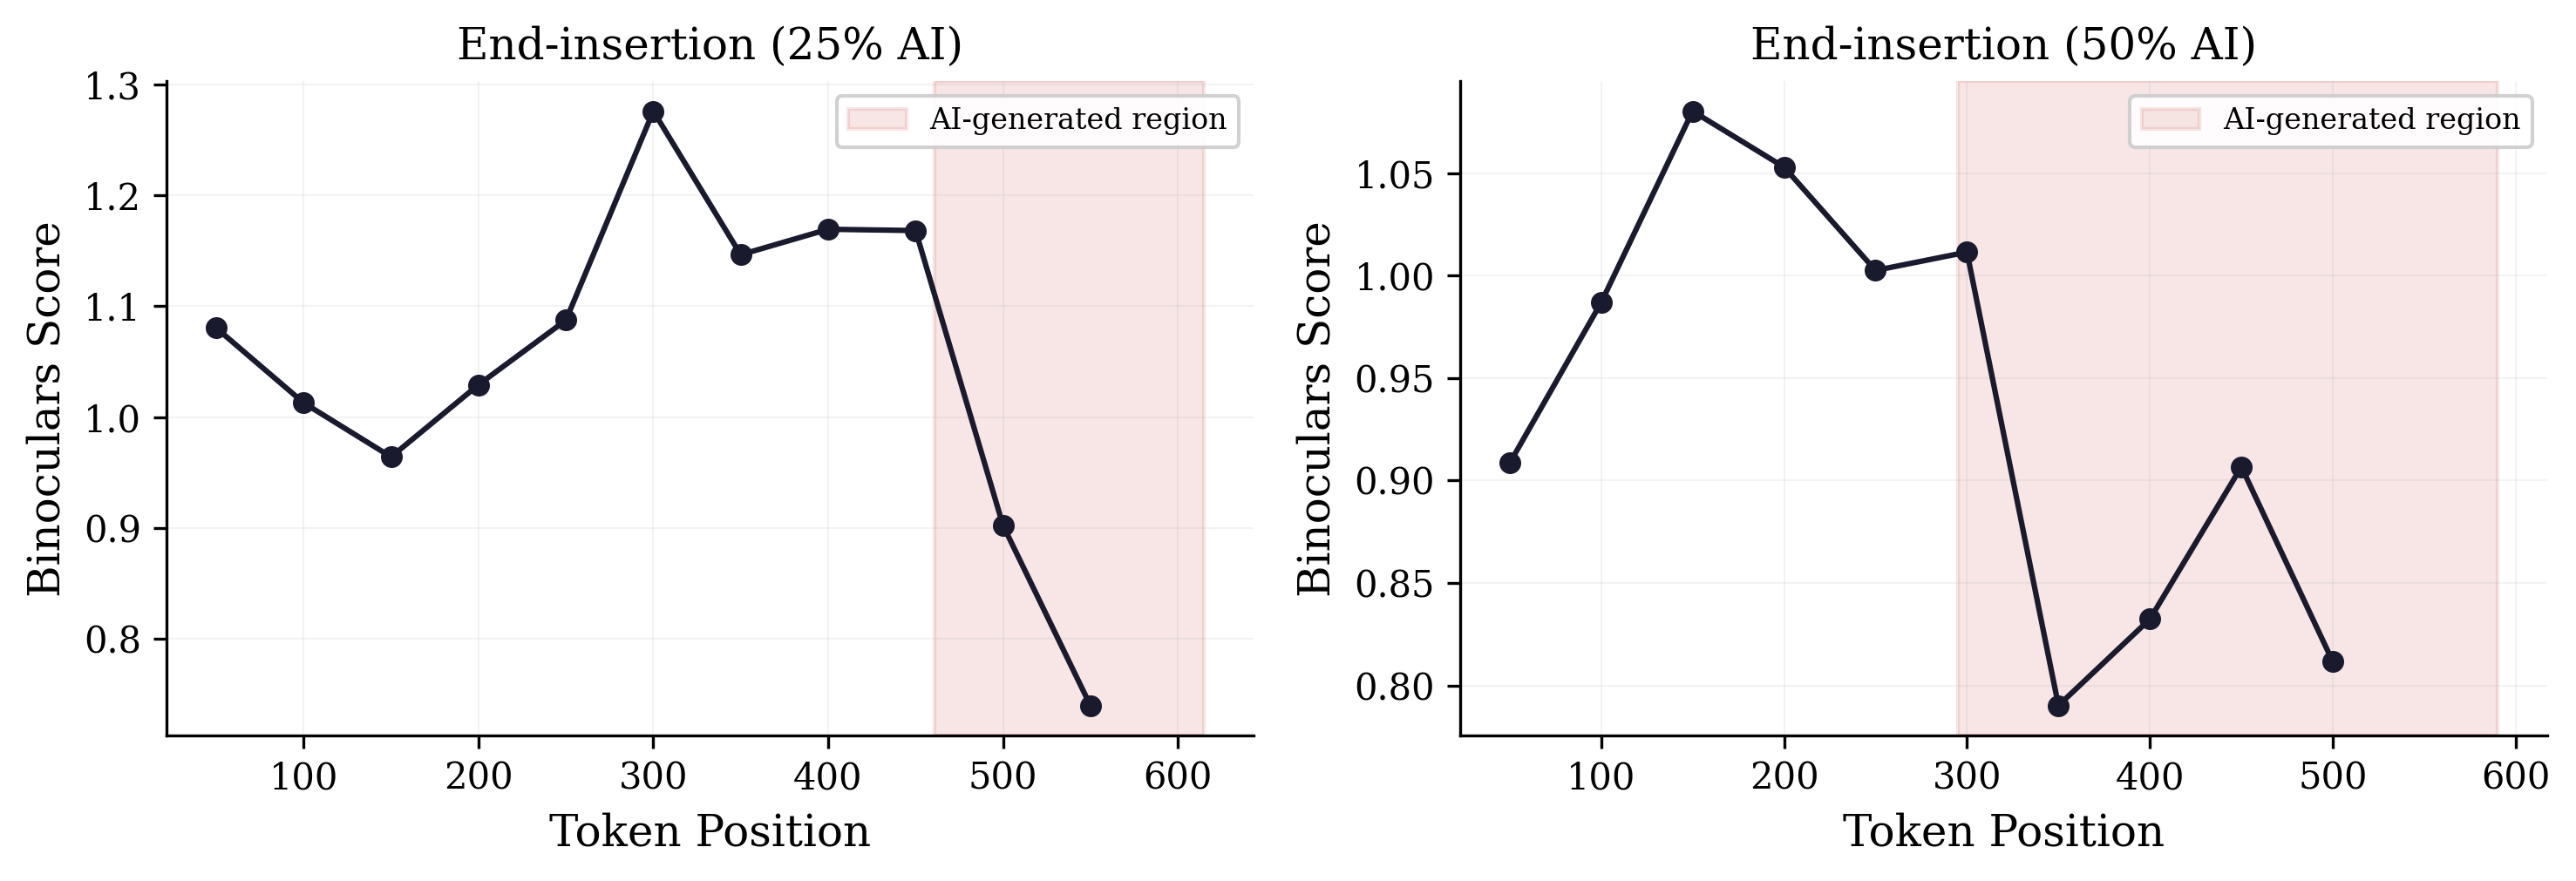
\includegraphics[width=\textwidth]{fig1.png}
\caption{\textbf{Segment-level detection visualization.} Binoculars scores computed over sliding windows ($W$=100, stride=50) on hybrid documents with AI content appended at the end. The shaded region indicates the ground-truth AI-generated portion. Scores drop noticeably upon entering the AI region, demonstrating that Ko-Binoculars can localize AI-generated segments within mixed documents.}
\label{fig:segment}
\end{figure}

Table~\ref{tab:segment} presents AI ratio estimation results on hybrid documents. Ko-Binoculars achieves an average MAE of 0.163, a 45.7\% reduction compared to random baseline (0.300). Performance is consistent across end-insertion and mid-insertion scenarios, demonstrating robustness to the position of AI-generated content.

\begin{table}[h]
\centering
\caption{\textbf{Segment-level AI ratio estimation error (MAE).} Ko-Binoculars with sliding window ($W$=100, stride=50) vs. random baseline. Both insertion scenarios yield identical results.}
\label{tab:segment}
\begin{tabular}{lcc}
\toprule
True AI Ratio & Ko-Bino & Random \\
\midrule
0\% & 0.121 & 0.500 \\
25\% & 0.090 & 0.250 \\
50\% & 0.175 & 0.000 \\
75\% & 0.205 & 0.250 \\
100\% & 0.225 & 0.500 \\
\midrule
Average & \textbf{0.163} & 0.300 \\
\bottomrule
\end{tabular}
\end{table}

\section{Analysis}

\subsection{NLL Dispersion and Sampling Temperature}

To understand why NLL dispersion serves as an effective detection signal, we investigate its relationship with sampling temperature. We generate texts using Qwen2.5-3B-Instruct at 15 temperature settings and measure the resulting NLL dispersion.As shown in Figure 2, NLL dispersion shows a clear increasing trend with temperature (Pearson $r = 0.73$, $p < 0.0001$), confirming that it captures generation uncertainty.

\begin{figure}[h]
\centering
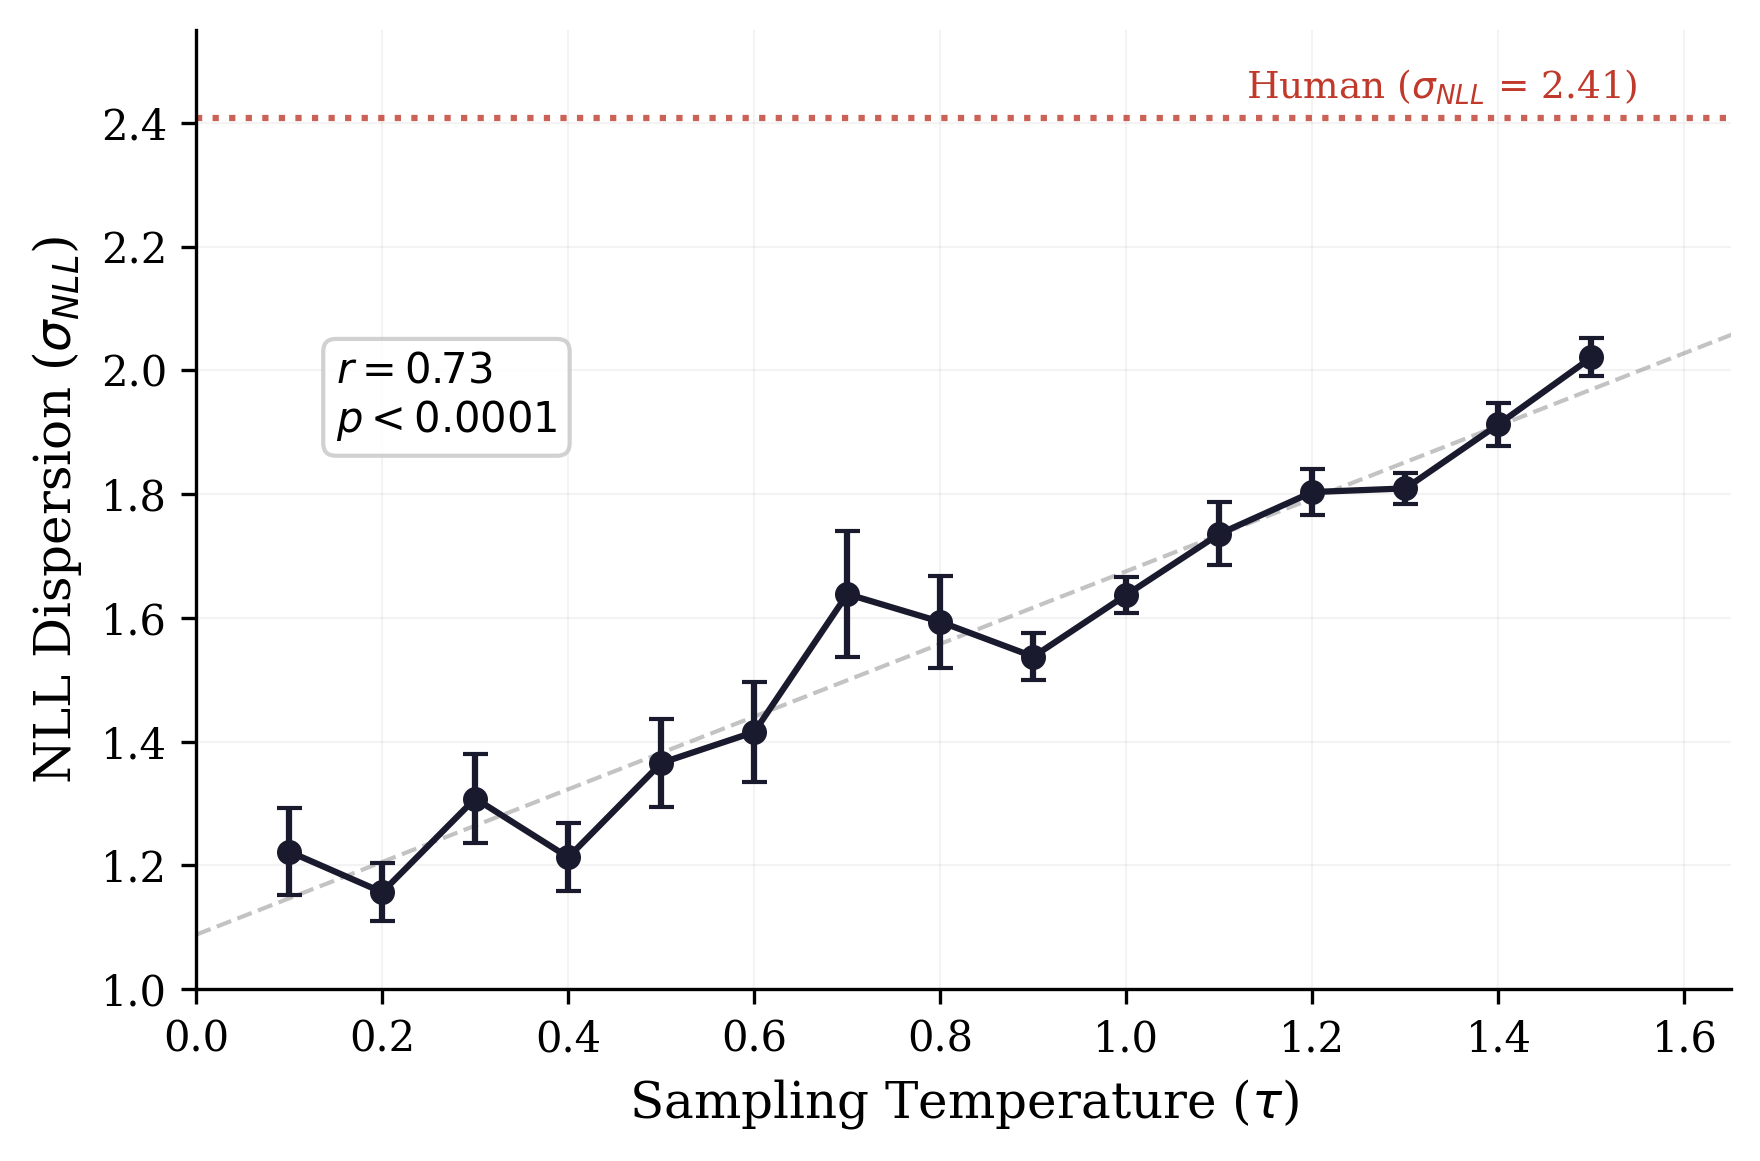
\includegraphics[width=0.7\textwidth]{fig2.png}
\caption{\textbf{NLL dispersion vs. sampling temperature.} Texts are generated at 15 temperature settings ($\tau \in [0.1, 1.5]$) and measured for NLL dispersion. A strong positive correlation is observed (Pearson $r = 0.73$, $p < 0.0001$). The red dashed line indicates the average human NLL dispersion (2.41), which exceeds all AI-generated samples, confirming that human writing exhibits higher token-level unpredictability than LLM outputs at any tested temperature.}
\label{fig:temperature}
\end{figure}


Using the fitted regression ($\tau = 0.677 \cdot \sigma_{\mathrm{NLL}} - 0.255$), we tentatively estimate the effective temperature of texts in the KatFish dataset. Human text corresponds to approximately 1.38, while AI-generated texts range from 1.05 (Solar) to 1.11 (Llama3.1). We note two important caveats: first, the human estimate involves extrapolation beyond the fitted range ($\tau \leq 1.5$) and should be interpreted as an approximate indicator rather than a precise measurement. Second, the regression was fitted using a single model (Qwen2.5-3B-Instruct), and the effective temperature concept may not transfer directly to texts generated by other LLMs with different architectures and sampling configurations. Nevertheless, the consistent gap of approximately 0.27 between human and AI dispersion values provides empirical support for using NLL dispersion as a detection signal. Importantly, this analysis also reveals a fundamental limitation: if LLMs generate text at sufficiently high temperatures, the NLL dispersion gap would narrow, making detection more difficult.

\subsection{Gated Fusion and Domain Recognition}

We analyze the gate values produced by the gated fusion mechanism across genres. The mean absolute z-score $|z|$ differs substantially: essay (1.83), poetry (1.28), and abstract (0.67). Measured by the ability to distinguish abstract from other genres using $|z|$ alone, the gate achieves an AUC of 83.58, confirming that the gating mechanism implicitly captures domain characteristics and adjusts signal reliance accordingly.

\section{Conclusion}

\subsection{Summary}

We presented Ko-Binoculars, a training-free framework that addresses the limitations of English-centric detection models by using Korean-optimized observer-performer pairs, improving ROC-AUC from 67.54 to 95.40. Furthermore, we introduced NLL Dispersion Calibration, leveraging the strong correlation ($r=0.73$) between NLL dispersion and sampling temperature to adaptively adjust scores. Finally, we extended this to segment-level detection, reducing AI ratio estimation error by 45.7\% compared to a random baseline.

\subsection{Limitations}

Our approach has several limitations. First, calibration degrades on the abstract genre, where human and AI writing styles exhibit similar NLL dispersion, likely due to the highly formulaic nature of academic writing and the limited number of human abstract samples. Second, the Min-Max normalization used for calibration introduces a potential source of information leakage. However, a Human-reference-only variant achieves comparable performance (87.93 vs. 88.14 ROC-AUC), suggesting that the observed improvements are not primarily driven by this effect. Third, our segment-level detection has only been evaluated on synthetically constructed hybrid documents, which may not fully reflect real-world mixed-authorship patterns.

\subsection{Future Work}

Promising directions include developing domain-adaptive calibration strategies that automatically detect and handle low-dispersion domains such as academic writing, extending the framework to other non-English languages using the fertility-based model selection heuristic, and evaluating segment-level detection on naturally occurring mixed-authorship documents.

\bibliographystyle{unsrt}
\bibliography{references}
% you can use .bib file to take care of your references.

\newpage
\appendix
\counterwithin{table}{section}

\section{Appendix: Team contributions}
\begin{itemize}
    \item \textbf{GyeongMin Bae}: Data preparation, Ko-Binoculars implementation, NLL dispersion analysis, and paper writing.
    \item \textbf{SeongHyeon Mun}: Multiplicative calibration, Gated fusion, Segment-level detection mechanism, and paper writing.
\end{itemize}

\section{Appendix: Dataset}
\begin{table}[h]
\centering
\caption{\textbf{KatFish dataset statistics.} The dataset contains human-written and AI-generated Korean texts across three genres. We follow the OOD evaluation protocol of KatFishNet: 20\% of human texts are held out as the test set (seed = 42), GPT-4o is excluded from evaluation, and detection performance is measured against Solar, Qwen2, and Llama3.1.}
\label{tab:dataset}
\begin{tabular}{lccccc}
\toprule
Genre & Human & GPT-4o & Solar & Qwen2 & Llama3.1 \\
\midrule
Essay & 205 & 181 & 140 & 181 & 88 \\
Abstract & 65 & 100 & 100 & 17 & 61 \\
Poetry & 200 & 189 & 189 & 189 & 189 \\
\midrule
Total & 470 & 470 & 429 & 387 & 338 \\
\bottomrule
\end{tabular}
\end{table}

\end{document}
